\chapter{Deep Kalman Filter}\label{sec:DKF}

The Kalman Filter is a well known model, widely used to denoise time series observations and 
make predictions. The latent variables form a Markov Chain, and all the probability distributions 
(ie encoder, decoder and transition model) are linear Gaussians. This allows to derive close form expressions for the solutions 
(the well-known Kalman filter and Kalman smoother).

In a \textbf{Deep Kalman Filter}, the temporal structure of the latent variables is still a Markov Chain. The probaility models are still Gaussians, but with parameters mean and covariance learnt by neural networks.

More specifically, the \gls{dag} describing a Deep Kalman Filter is:

\begin{figure}[h]
    \centering
    % \includegraphics[width=0.5\linewidth]{}
    \label{fig:graphical_model_dkf}
\begin{tikzpicture}[
    HIDDEN/.style={circle, draw=black!0, thin, minimum size=10mm},
    UNOBS/.style={circle, draw=black!80, thin, minimum size=10mm},
    OBS/.style={circle, draw=black!80, fill=gray!50, thin, minimum size=10mm}
]
% nodes
\node[HIDDEN] (a) {$...$};
\node[UNOBS] (z_t_1) [right= of a] {$z_{t-1}$} edge[<-, thin] (a);
\node[UNOBS] (z_t)  [right= of z_t_1] {$z_{t}$} edge[<-, thin] (z_t_1);
\node[UNOBS] (z_t_p1) [right= of z_t] {$z_{t+1}$} edge[<-, thin] (z_t);
\node[HIDDEN] (e) [right= of z_t_p1] {$...$} edge[<-, thin] (z_t_p1);
\node[OBS] (x_t_1) [below= of z_t_1] {$x_{t-1}$} edge[<-, thin] (z_t_1);
\node[OBS] (x_t) [below= of z_t] {$x_{t}$} edge[<-, thin] (z_t);
\node[OBS] (x_t_p1) [below= of z_t_p1] {$x_{t+1}$} edge[<-, thin] (z_t_p1);
\end{tikzpicture}
\caption{Probabilistic model of a Deep Kalman Filter}
\end{figure}

It is then particularly useful to use D-separation on the \gls{dag} to simplify the general \gls{dvae} expressions \ref{gen_model_dvae} and \ref{inf_model_dvae}. Conditioning on $z_t$ and $z_{t-1}$ drives:
\begin{align}
    p_{\theta_x}(x_t \vert x_{1:t-1}, z_{1:t}) &= p_{\theta_x}(x_t \vert z_t) \\
    p_{\theta_z}(z_t \vert z_{1:t-1}, x_{1:t}) &= p_{\theta_z}(z_t \vert z_{t-1}) \\
    \label{dkf_posterior}
    q_{\phi}(z_t \vert z_{1:t-1}, x_{1:T}) &= q_{\phi}(z_t \vert z_{t-1}, x_{t:T}) 
\end{align}

We then choose Gaussian distributions for $p_{\theta_x}, p_{\theta_z}$ and $q_\phi$, with mean and diagonal covariance, learnt by neural networks.
\begin{align}
    p_{\theta_x}(x_t \vert z_t) &= \NNdiag{x_t}{\mu_{\theta_x}(z_t)}{\sigma_{\theta_x}^2(z_t)}\\
    p_{\theta_z}(z_t \vert z_{t-1}) &= \NNdiag{z_t}{\mu_{\theta_z}(z_{t-1})}{\sigma_{\theta_z}^2(z_{t-1})}\\
    q_{\phi}(z_t \vert z_{t-1}, x_{t:T}) &= \NNdiag{z_t}{\mu_{\phi}(z_{t-1}, x_{t:T})}{\sigma_{\theta_z}^2(z_{t-1},x_{t:T})}
\end{align}
Some other formulations of the approximate posterior (encoder) are possible. For example:
\begin{align*}
    q_{\phi}(z_t \vert z_{t-1}, x_t) \\
    q_{\phi}(z_t \vert z_{1:t}, x_{1:t}) \\
    q_{\phi}(z_t \vert z_{1:T}, x_{1:T})
\end{align*}
We have chosen \ref{dkf_posterior} for the implementation, as it has the same formulation as the true posterior and respects the corresponding dependencies.

Taking note that:
\begin{align*}
    q_{\phi}(z_{1:t} \vert x_{1:T}) = q_{\phi}(z_{1:t-1} \vert z_t, x_{1:T}) q_{\phi}(z_t \vert x_{1:T})
\end{align*}
And using D-Separation, the \gls{elbo} \ref{vlb_dvae} simplifies into:
\begin{align}
    \VLB &= \sum_{t=1}^T \E{q_\phi(z_{1:t} \vert x_{1:T})} \log{p_{\theta_x}(x_t \vert z_t)} - \sum_{t=1}^T \E{q_\phi(z_{1:t-1} \vert x_{1:T})} \KL{q_{\phi}(z_t \vert z_{t-1}, x_{t:T})}{p_{\theta_z}(z_t \vert z_{t-1})} \\
    &= \sum_{t=1}^T \E{q_\phi(z_{t} \vert x_{1:T})} \log{p_{\theta_x}(x_t \vert z_t)} - \sum_{t=1}^T \E{q_\phi(z_{t-1} \vert x_{1:T})} \KL{q_{\phi}(z_t \vert z_{t-1}, x_{t:T})}{p_{\theta_z}(z_t \vert z_{t-1})}
\end{align}

As a summary:
\begin{tcolorbox}[colback=blue!5!white,colframe=black!75!black,title=Deep Kalman Filter]
\begin{itemize}
    \item \textbf{generative model}
    \begin{align}
        \label{gen_model_dkf}
        p_{\theta_x}(x_t \vert z_t) &= \NNdiag{x_t}{\mu_{\theta_x}(z_t)}{\sigma_{\theta_x}^2(z_t)}\\
        p_{\theta_z}(z_t \vert z_{t-1}) &= \NNdiag{z_t}{\mu_{\theta_z}(z_{t-1})}{\sigma_{\theta_z}^2(z_{t-1})}
    \end{align}
    \item \textbf{inference model}
    \begin{align}
        \label{inf_model_dkf}
        q_{\phi}(z_t \vert z_{t-1}, x_{t:T}) &= \NNdiag{z_t}{\mu_{\phi}(z_{t-1}, x_{t:T})}{\sigma_{\theta_z}^2(z_{t-1},x_{t:T})}
    \end{align}
    \item \textbf{\gls{vlb} for training}
    \begin{align}
        \label{vlb_dkf}
        \VLB &= \sum_{t=1}^T \E{q_\phi(z_{t} \vert x_{1:T})} \log{p_{\theta_x}(x_t \vert z_t)} - \sum_{t=1}^T \E{q_\phi(z_{t-1} \vert x_{1:T})} \KL{q_{\phi}(z_t \vert z_{t-1}, x_{t:T})}{p_{\theta_z}(z_t \vert z_{t-1})}
    \end{align}
\end{itemize}
\end{tcolorbox}

The $\KL{q_\phi}{p_{\theta_z}}$'s have a close form, as the two distributions are Gaussians (see \ref{sec:KL-two-exponential-family-distributions})

From a code stand-point, following \cite{girin_dynamical_2022}, we have used forward \gls{lstm} to encode sequences such as $x_{1:t}$, and backward \gls{lstm} to encode sequences such as $x_{t:T}$, as inputs into the \gls{mlp} parametrizing the distributions. 

For example:
\begin{align*}
    \overleftarrow{g_t} &= \text{Backward LSTM}(\overleftarrow{g_{t+1}}, x_t) \,\, (\text{encodes} \,\, x_{t:T}) \\
    q_{\phi}(z_t \vert z_{t-1}, x_{t:T}) &= \NNdiag{z_t}{\mu_{\phi}(z_{t-1}, \overleftarrow{g_t})}{\sigma_{\phi}^2(z_{t-1}, \overleftarrow{g_t})}
\end{align*}



The PyTorch implementation is schematized below (with $B$ batch size, $T$ the length of the data sequence, $D_x$ the dimension 
of the observation space, $D_z$ the dimension of the latent space):

\newpage
%
%
%------- DEEP KALMAN FILTER ------------------------------
%
%

\begin{landscape}
\begin{figure}
\begin{centering}
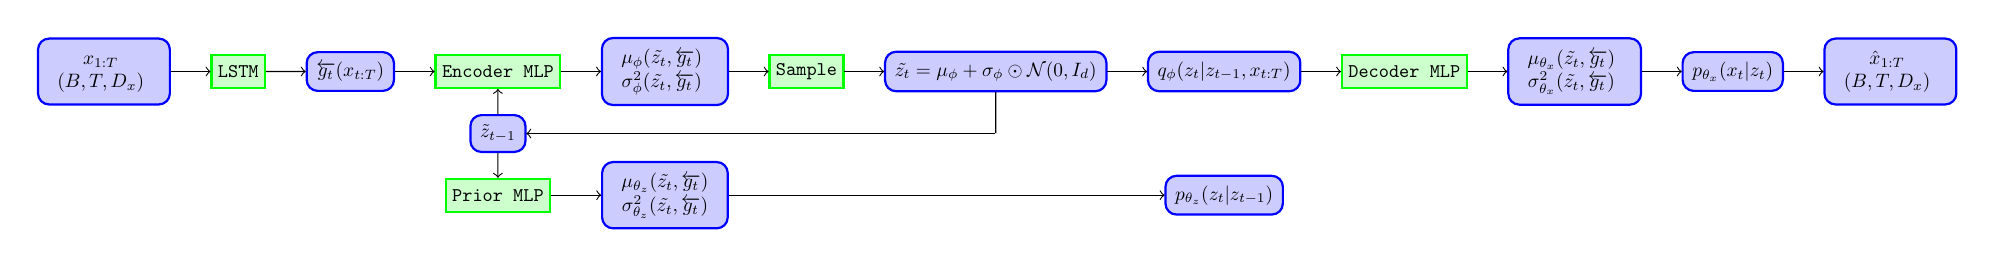
\begin{tikzpicture}[
    scale=0.70,
    every node/.style={scale=0.70},
    torch/.style={
        rectangle, 
        minimum size=6mm, 
        thick, 
        draw=green!100, 
        fill=green!20, 
        font=\ttfamily
        },
    math/.style={
        rectangle, 
        % minimum height=1cm,
        % minimum width=2cm,
        rounded corners, 
        thick, 
        draw=blue!100,
        fill=blue!20,
        align=center,
        anchor=center,
        inner sep=5pt
        },
    point/.style={
        circle,
        inner sep=0pt,
        minimum size=0pt,
        }
    ]
\matrix[row sep = 1mm, column sep=5mm] {
% first row
\node[math] (xt) {
    $\begin{array}{c}
            x_{1:T} \\
            (B,T,D_x)
    \end{array}$
}; & 
\node[torch] (lstm) {LSTM}; & 
\node[math] (gt) {$\overleftarrow{g_t}(x_{t:T})$}; &
\node[torch] (enco) {Encoder MLP}; &
\node[math] (phi) {
    $\begin{array}{c}
            \mu_{\phi}(\tilde{z_t}, \overleftarrow{g_t}) \\
            \sigma_{\phi}^2(\tilde{z_t}, \overleftarrow{g_t})
    \end{array}$
}; &
\node[torch] (sample) {Sample}; &
\node[math] (z_tilde) {$\tilde{z_t} = \mu_{\phi} + \sigma_{\phi} \odot \mathcal{N}(0, I_d)$}; &
\node[math] (q_phi) {$q_{\phi}(z_t \vert z_{t-1}, x_{t:T})$}; &
\node[torch] (deco) {Decoder MLP}; &
\node[math] (theta_x) {
    $\begin{array}{c}
        \mu_{\theta_x}(\tilde{z_t}, \overleftarrow{g_t}) \\
        \sigma_{\theta_x}^2(\tilde{z_t}, \overleftarrow{g_t})
    \end{array}$
}; &
\node[math] (p_theta_x) {$p_{\theta_x}(x_t \vert z_t)$}; &
\node[math] (x_hat) {
    $\begin{array}{c}
            \hat{x}_{1:T} \\
            (B,T,D_x)
    \end{array}$
}; \\
%second row
& & & \node[math] (z_t_1) (z_t_1) {$\tilde{z}_{t-1}$}; & & & \node[point] (coin) {}; & & &; \\
%third row
& & & \node[torch] (prior) {Prior MLP}; &
\node[math] (theta_z) {
    $\begin{array}{c}
            \mu_{\theta_z}(\tilde{z_t}, \overleftarrow{g_t}) \\
            \sigma_{\theta_z}^2(\tilde{z_t}, \overleftarrow{g_t})
    \end{array}$}; & & &
\node[math] (p_theta_z) {$p_{\theta_z}(z_t \vert z_{t-1})$}; &
& & \\
};
\path   (xt) edge [->, thin] (lstm)
        (lstm) edge [->, thin] (gt)
        (gt) edge [->, thin] (enco)
        (enco) edge [->, thin] (phi)
        (phi) edge [->, thin] (sample)
        (sample) edge [->, thin] (z_tilde)
        (z_tilde) edge [->, thin] (q_phi)
        (q_phi) edge[->, thin] (deco)
        (deco) edge [->, thin] (theta_x)
        (theta_x) edge [->, thin] (p_theta_x)
        (p_theta_x) edge [->, thin] (x_hat)
        (z_t_1) edge [->, thin] (enco)
        (prior) edge [<-, thin] (z_t_1)
        (theta_z) edge [<-, thin] (prior)
        (theta_z) edge[->, thin] (p_theta_z)
        (z_tilde) edge [-, thin] (coin)
        (coin) edge [->, thin] (z_t_1);
\end{tikzpicture}

% --- Loss DKF
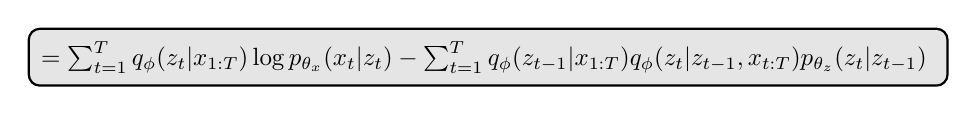
\begin{tikzpicture}[
    scale=0.90,
    every node/.style={scale=0.90},
    math/.style={
        rectangle, 
        % minimum height=1cm,
        % minimum width=2cm,
        rounded corners, 
        thick, 
        draw=black!100,
        fill=gray!20,
        align=center,
        anchor=center,
        inner sep=5pt
        },
    ]
    \node[math] {
            $\VLB = \sum_{t=1}^T \E{q_\phi(z_{t} \vert x_{1:T})} \log{p_{\theta_x}(x_t \vert z_t)} - \sum_{t=1}^T \E{q_\phi(z_{t-1} \vert x_{1:T})} \KL{q_{\phi}(z_t \vert z_{t-1}, x_{t:T})}{p_{\theta_z}(z_t \vert z_{t-1})}$
    };
\end{tikzpicture}

\end{centering}
\caption{Deep Kalman Filter Model Architecture}
\end{figure}
\end{landscape}